\documentclass[12pt]{article}
\usepackage{fullpage}
\usepackage[a4paper, margin=2cm, bottom=3cm]{geometry}
\usepackage{graphicx}
\usepackage{titling}
\setlength{\droptitle}{-60pt}
\usepackage{url}
\usepackage{enumerate}
\usepackage{hyperref}

\usepackage[T1]{fontenc} %needed for French quotes
\usepackage{ucs}
\usepackage[english, francais]{babel}
\usepackage[utf8x]{inputenc}
\newcommand{\en}[1]{\selectlanguage{english}#1\selectlanguage{francais}}


\newcommand{\ttt}{\textit{Tic-tac-toe}}
\newcommand{\cf}{\textit{Puissance 4}}
\newcommand{\oth}{\textit{Othello}}
\newcommand{\progalgo}[1]{<<~Programmation et Algorithmique #1~>>}

\title{Rapport de projet (BA1 informatique, UMONS)}
\author{Mathieu Leclerq, Guillaume Huysmans}
\hypersetup{pdfauthor={Mathieu Leclerq, Guillaume Huysmans},
            pdftitle={Projet d'informatique (BA1 à l'UMONS) - Boîte à jeux},
            pdfsubject={rapport, documentation},
            pdfkeywords={rapport, documentation}}
\begin{document}
\maketitle
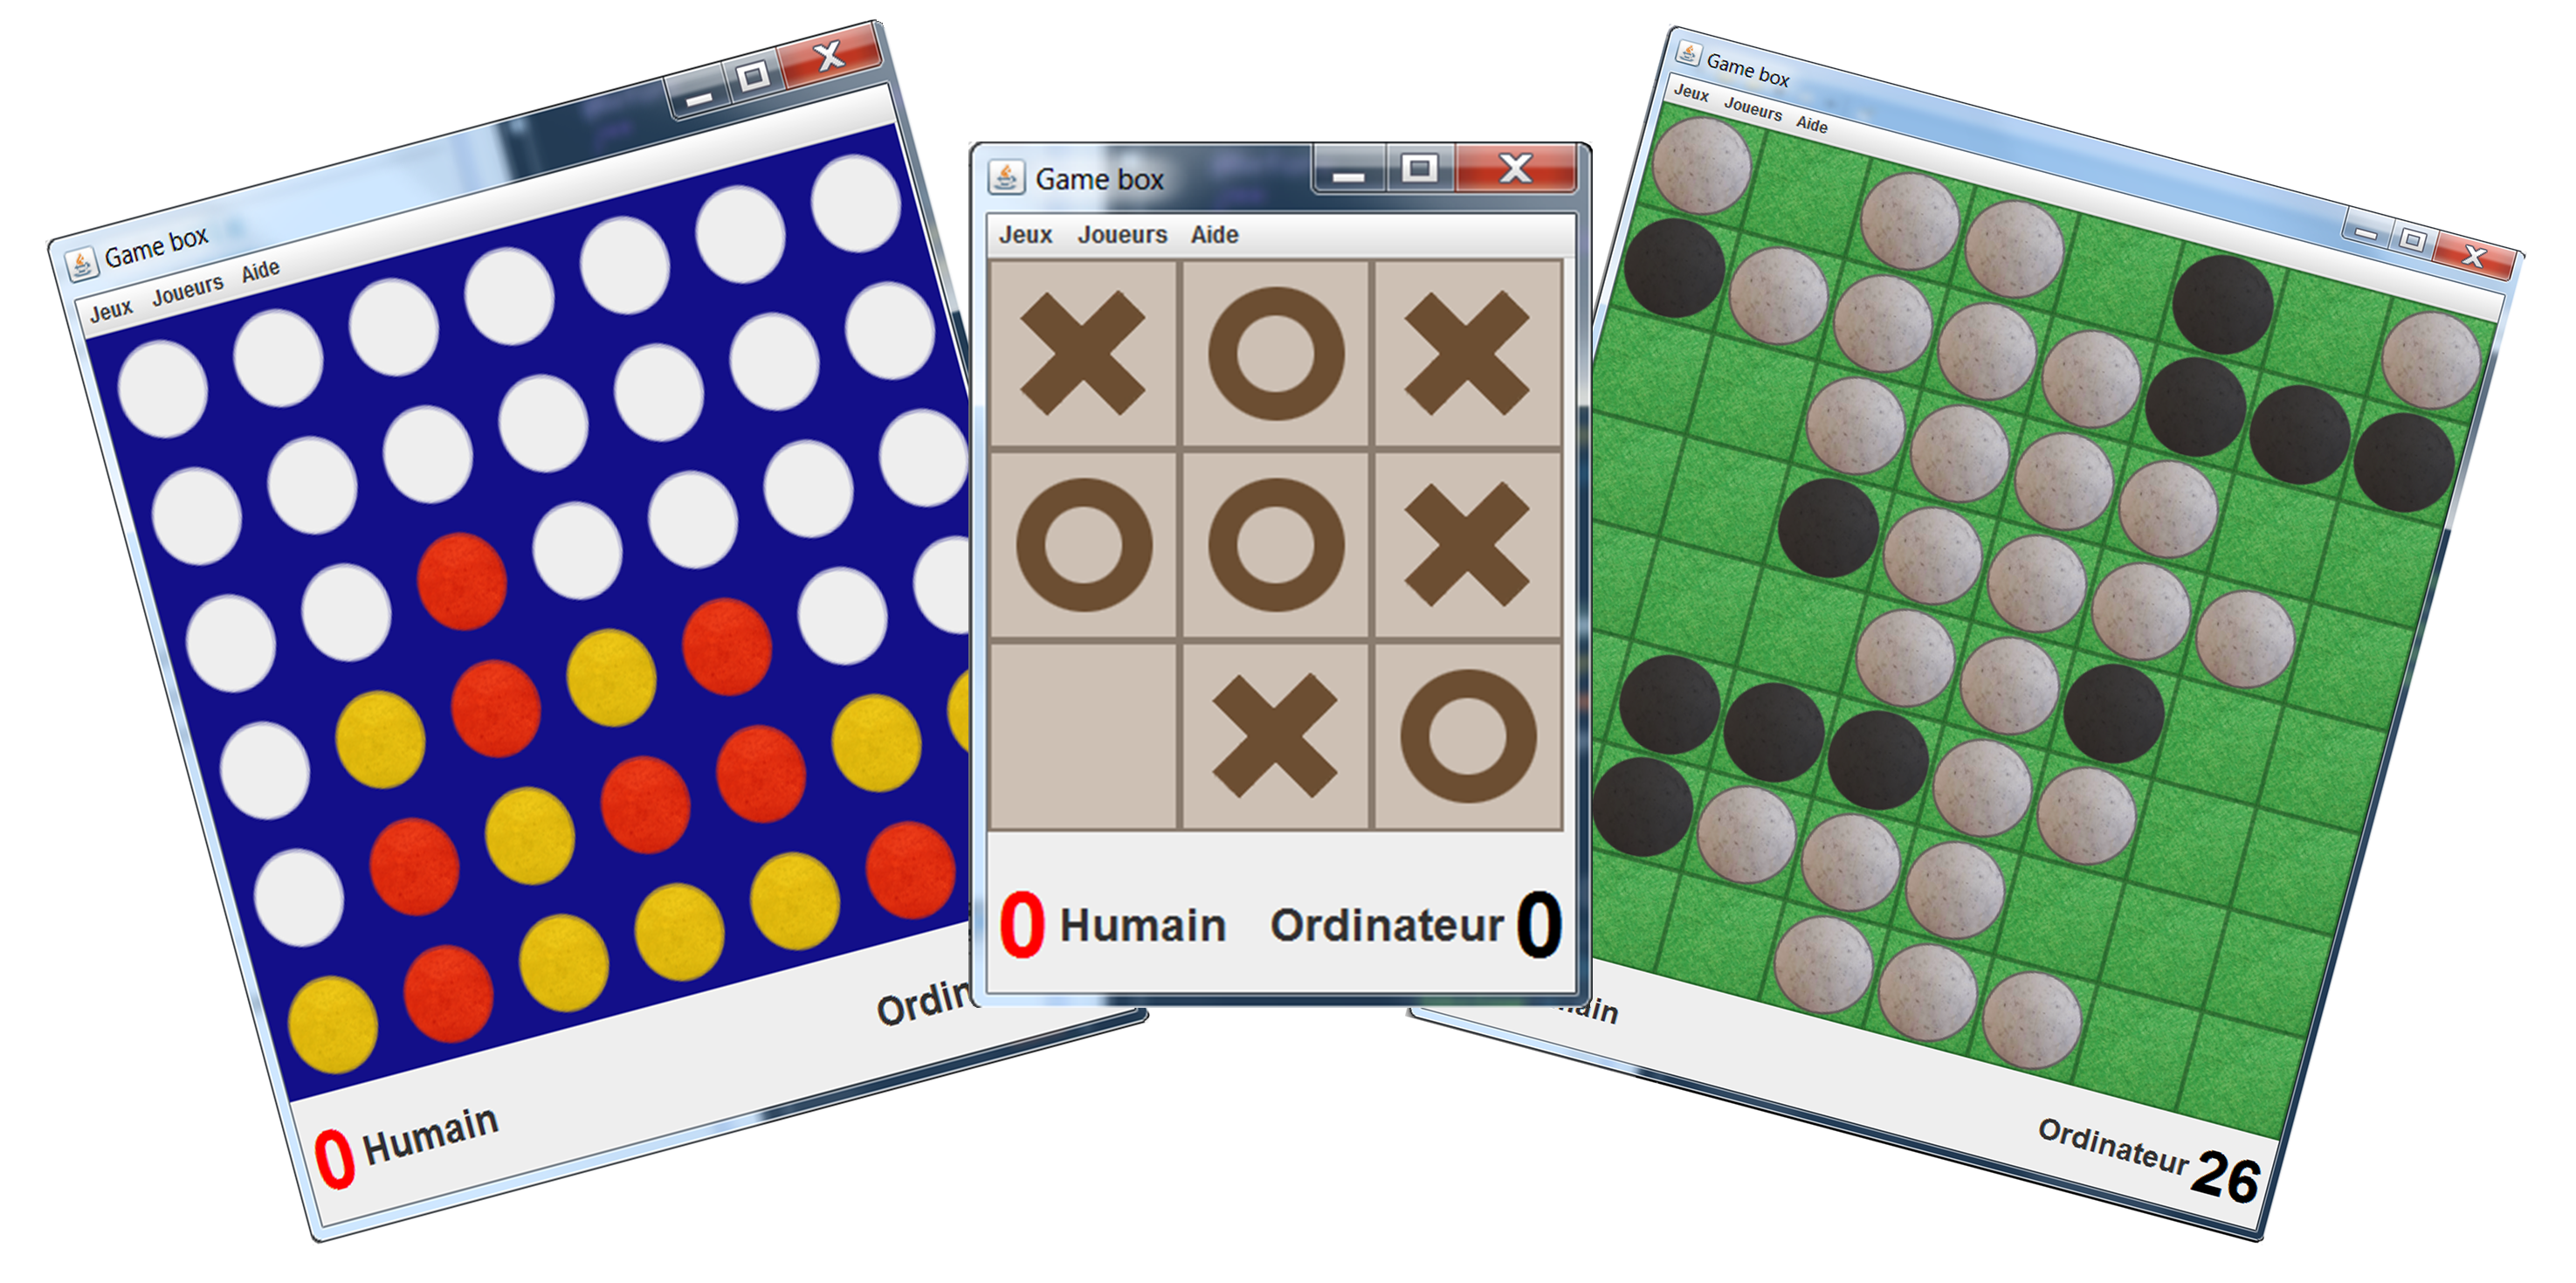
\includegraphics[width=\textwidth]{../cover.png}
\tableofcontents
\newpage

\section{Introduction}
Il nous a été demandé de développer en binôme une <<~boîte à jeux~>> en Java 6, c'est-à-dire 
un moteur de jeu doté d'une interface graphique capable de faire fonctionner plusieurs jeux 
de plateau : \ttt{}, \cf{} et \oth. C'était l'occasion de montrer les~compétences développées 
en cours de \progalgo{1}{} et les~notions de programmation orientée objet 
abordées en \progalgo{2} et de s'initier aux bonnes pratiques du développement à plusieurs.
\section{Points positifs}
TODO

\section{Choix argumentés}

\subsection{Organisation interne}
Le même objet est utilisé pour représenter le~plateau de tous les~jeux. Ce~plateau n'est jamais manipulé directement par ces~derniers :
les~objets représentant les~jeux génèrent des listes de coups possibles qui seront ensuite utilisés par les différentes intelligences artificielles.
Pour savoir si un~mouvement est autorisé, il nous suffit de vérifier qu'il appartient à cette~liste. 

Du fait que les~jeux proposent tous une~liste de coups autorisés par les~règles, les~intelligences artificielles sont indépendantes des jeux :
il suffit de modéliser les~différents types de mouvements et leurs~conséquences pour permettre \emph{à la fois} à un~joueur humain et au logiciel de jouer !

Le~jeu de \ttt{} et \cf{} ont une~caractéristique commune : les~conditions de victoire sont identiques, seul le~nombre de jetons diffère !
\cf{} ne fait qu'ajouter une~contrainte lorsqu'un~jeton est joué, c'est pourquoi il hérite de \ttt.

L'historique est géré sous la~forme d'une~pile : on ne peut défaire un~mouvement que lorsque c'est le~dernier effectué. 
Les~intelligences artificielles s'en servent abondamment pour explorer les différentes possibilités. 
Cela implique que l'affichage ainsi que les événements ne doivent pas toujours être mis à jour : 
lorsqu'une~IA <<~réfléchit~>>, les~mouvements effectués ne le sont pas réellement (ils sont \emph{virtuels})...

Les~succès et les~différents messages (sonores ou textuels) sont gérés à travers un~seul mécanisme : 
les~événements. Ces~derniers sont constitués de plusieurs compteurs nommés, mis à jour par le~jeu lui-même. 

L'utilisation du design patern \texttt{Observer} nous évite des incohérences entre l'interface graphique et l'état interne des jeux.

La~sérialisation nous a permis de facilement sauvegarder et enregistrer les~parties en cours et les~profils des joueurs. 
Les~classes composant le~design pattern \texttt{Observer} ont cependant dû être réécrites puisqu'\texttt{Observable} n'est pas sérialisable, 
ce qui nous empêchait de sauvegarder les~liens entre les différentes conditions et le~jeu en cours d'exécution.


\subsection{Sauvegarde et chargement}
Le fait qu'un objet \texttt{JPanel} puisse être sérialisé peut apparaître comme une solution miracle à ce problème 
mais nous avons pourtant pris la~décision de ne pas faire reposer notre mécanisme de sauvegarde là-dessus.

Premièrement, l'interface graphique doit pouvoir évoluer sans pour autant interférer avec les~sauvegardes effectuées auparavant : 
qui voudrait mettre à jour son~jeu et voir disparaître ses~profils de joueurs ?

Ensuite, nous sommes capables de recréer tous les~composants de l'interface graphique nécessaires à l'utilisation d'un jeu 
à partir d'une instance sauvegardée d'un objet \texttt{Game} : une énumération associant la~classe de chaque jeu jouable 
aux informations nécessaires à la~création du~\texttt{BoardPanel} correspondant est chargée dans le~constructeur de \texttt{Main}, 
il nous suffit de trouver parmi les~éléments celui qui correspond à la~classe de l'objet sauvegardé ! C'est également cette même structure 
%FIXME orthographe ? <<~sélection de jeux~>> ??
qui nous permet de construire le menu de sélection de jeu entièrement à la volée.


\subsection{Intelligences artificielles}
Comme il nous était demandé d'implémenter plusieurs <<~intelligences artificielles~>>, 
nous en avons choisi trois, classées ici par niveau selon l'ordre croissant :

\begin{enumerate}
	\item \emph{Hasard} : elle sélectionne un~coup au~hasard parmi les~coups légaux.
    \item \emph{Premier} : elle sélectionne le premier coup légal de la~liste. Le~balayage est fait,
    \begin{itemize}
        \item pour \oth{} et \ttt{} : de gauche à droite et de haut en bas.
        \item pour \cf{} : de gauche à droite.
    \end{itemize}
    \item \emph{Negamax} : elle sélectionnera le meilleur coup possible en simulant les~coups de son~adversaire sur plusieurs niveaux de récursivité.
\end{enumerate}
\section{Zoom sur l'algorithme Negamax}

Dans un jeu à somme nulle
\footnote{Un jeu à somme nulle est un jeu dans lequel la~somme des valeurs des pertes et des gains de chaque joueur est nulle. Lorsqu'un joueur a un avantage de $n$ points sur l'autre, ce dernier a un désavantage de $-n$ points.}, 
on peut imaginer une stratégie gagnante pour chaque joueur (que nous nommerons Alice et Bob) : 
\begin{itemize}
	\item Alice doit chercher à maximiser ses profits (minimiser ceux de Bob).
	\item Bob doit chercher à maximiser ses profits (minimiser ceux d'Alice).
\end{itemize}

Malheureusement, l'espace de recherche est trop important pour être exploré entièrement : 
nous devons nous limiter à une certaine profondeur. Dans notre~code, on <<~creuse~>> jusqu'à 
6~niveaux (6~coups joués à tour de rôle).

L'ensemble des situations de jeu examinées par l'algorithme Negamax 
peut être représenté sous la~forme d'un arbre dans lequel :
\begin{itemize}
	\item Chaque noeud représente une situation de jeu.
    \item Chaque situation non finale a des descendants.
\end{itemize}

La~valeur d'un noeud correspondra au score obtenu par le~joueur actuel; elle vaudra... :
\begin{itemize}
	\item le~score final si la~partie est terminée ou si le~niveau maximal de récursion a été atteint.
    \item le meilleur score obtenu en essayant chaque mouvement légal, en se rappelant récursivement 
            et en inversant la~valeur retournée puisque celle-ci correspond au score du~joueur adverse 
            (puisqu'il n'y a dans nos~jeux que deux~joueurs).
\end{itemize}

Le meilleur coup à jouer est celui qui rapporte le plus de points.
\section{Répartition du travail}
\begin{enumerate}

\item Guillaume Huysmans
\begin{enumerate}
	\item Système de succès et plus généralement, d'événements.
    \item Gestion des mouvements et de leur historisatioon.
    \item Interface graphique :
    \begin{enumerate}
        \item plateau de jeu
    \end{enumerate}
\end{enumerate}

\item Mathieu Leclercq
\begin{enumerate}
	\item Création de toutes les~textures et icônes.
    \item Interface graphique : 
    \begin{enumerate}
        \item barre d'informations
        \item sélection des IA
    \end{enumerate}
\end{enumerate}

\end{enumerate}

\section{Apports personnels}

\subsection{Mathieu Leclercq}
Pour ma part, j'ai apprécié le~fait de devoir travailler en groupe et de concevoir un~projet dans son~entièreté,
devoir penser aux moyens les plus efficaces pour que le~programme respecte le~cahier des charges. 
Ce~projet m'a aussi permis d'utiliser certaines notions de Java vues au cours et que l'on n'avait pas encore eu 
l'occasion d'utiliser durant les séances de travaux pratiques.   

\subsection{Guillaume Huysmans}
Ce~projet n'était pas pour moi le~premier mais il m'a apporté un~éclairage nouveau sur le~développement logiciel : 
tout d'abord, je n'avais jamais développé un projet complet ni en un~langage orienté objet, ni avec un autre développeur. 
Cela implique une toute autre manière de travailler : il faut obligatoirement s'interroger en profondeur (et se mettre d'accord) 
sur la~structure du projet avant de commencer à coder afin d'éviter tout conflit (par exemple, un~changement radical 
de fonctionnement qui impliquerait la~réécriture de toute une~partie du~code). 
L'UML produit lors de cette~phase d'analyse m'a été d'une~grande aide pour me tenir à ce qui avait été prévu. 
Le~code que nous écrivons doit en outre être suffisamment documenté pour éviter toute perte de temps.
Heureusement, la~POO rend bien plus facile le~développement collaboratif à travers l'encapsulation : ce qui se passe à l'intérieur 
d'un~objet n'a pas d'influence sur le~reste du code, ce qui permet d'effectuer des modifications sans tout <<~casser~>>. 
Ce jeu nous a également donné l'occasion d'apprendre à utiliser efficacement 
un~VCS\footnote{\emph{Version Control System}, système de contrôle de versions} 
afin de coordonner notre~travail le plus efficacement possible : la~synchronisation manuelle des codes sources par e-mail ou 
clé USB est un~travail lourd, difficile, source d'erreurs et d'énormes frustrations.
\section{Points négatifs}
TODO

\section{Bogues connus}
\begin{itemize}

	\item Lorsqu'on sélectionne une~IA et que l'on clique sur \textit{Annuler}, 
            elle semble sélectionnée dans le menu alors qu'elle ne l'est pas.
            
    %\item XXX
    
\end{itemize}

\appendix
\section{Annexe : UML}

\begin{figure}[ht]
\centering
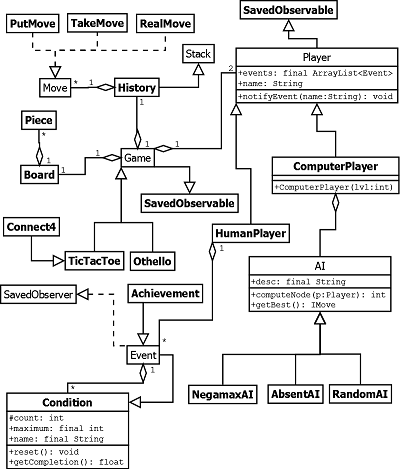
\includegraphics{../uml_global.png}
\caption{Diagramme de classes global}
\label{fig:umlGlobal}
\end{figure}
\begin{figure}[ht]
\centering
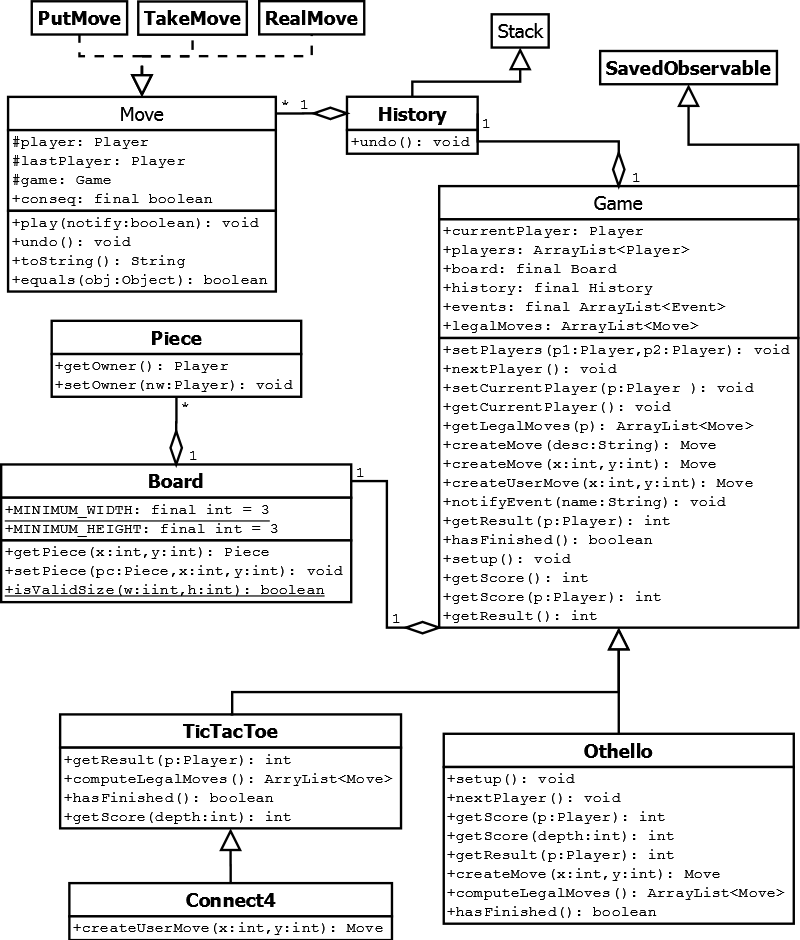
\includegraphics{../uml_Game.png}
\caption{Diagramme de classes axé sur \texttt{Game}}
\label{fig:umlGame}
\end{figure}

\end{document}
